
\section{Tools Used}

\subsection{Modeling \& Simulation}\label{intro:sim}

\subsection{Supply Chain Modeling}
The interactions that we wish to model are those of supply and demand. Certain
facilities need some sort or raw or processed material that other facilities
produce. The fuel cycle is more complicated than this simple statement, though,
because facilities are connected through recycled fuel. Even with such a
complication, the notion of a generic fuel cycle, i.e., from the perspective of
facilities that supply and demand material, quickly begins to look like a supply
chain model. There is a growing literature of agent-based supply chain modeling
\cite{swaminathan_modeling_1998,julka_agent-based_2002,van_der_zee_modeling_2005,chatfield_multi-formalism_2007,holmgren_agent_2007}.
The general premise of these types of models is that individual facilities have
a notion of their needs (i.e., their demands) and can express to the system
these needs at the required time. There is heavy use of inventory policy to
determine the correct amount of material inventory that is needed and the
correct time to request a resupply. In general, a facility may be comprised of
many agents, e.g., an ordering agent, a stocking agent, a forecasting agent,
etc. Such an approach has not heretofore been attempted for the nuclear fuel
cycle and opens up a variety of doors. For example, reactor facilities could be
allowed to be fueled by multiple fuel types (e.g., UOX or MOX), and decide which
type to choose based on the simulation environment. However, due to the
fungibility of material in the fuel cycle and its multicommodity nature, many
questions remain about how to describe the materials to be traded and the
markets on which they will be traded. 

The notion of regional modeling in fuel cycle simulation has to date been a
secondary concern. Certain simulators attempt to model it explicitly, e.g.,
DESAE \cite{iaea_nuclear_2010}. Other simulators have attempted to add the
capability at some point after their simulator had already been developed, e.g.,
VISION and COSI. A discussion of these capabilities follows in
\S\ref{sec:simulators}. Some semblance of this capability is needed if one is to
incorporate outside effects on a domestic fuel cycle. Furthermore, a robust
capability is required if one wishes to actually investigate dynamic
interactions amongst regional entities. Again, a full treatment of this sort of
regional interaction would require international relations models, most of which
can be found in the cross-cutting disciplines of economics, political science,
and game theory. The primary solution technique is called Nash Equilibrium, and
effectively describes an optimal solution as follows: given a set of players,
states, preferences, and actions, all players choose an action such that any
single player's deviation from that actions results in a state of lower
preference for that player (thus no player has an incentive to deviate)
\cite{mccarty_political_2007}. There also exists a body of literature that
examine Nash Equilibria in the context of optimal flow models
\cite{mazumdar_fairness_1991,nagurney_supply_2002,song_nash_2002}. However, the
complexity of such models quickly brings them out of the scope of our needs,
i.e., dynamic modeling of multi-lateral scenarios ranging 100+ years in a short
computation time ($\sim 10^0 - 10^1$ minutes). Accordingly, a market resolution mechanism
has been proposed that allows for interaction amongst the various facilities and
managing entities (e.g., their regions). In order to inform a cardinal
preference \cite{strotz_cardinal_1953} relation for a facility over its possible
supply materials. The full approach is outlined in sections
\S\ref{sec:agent-interaction} and \S\ref{sec:gfctp}.

\subsection{Transportation Problems \& Mathematical Programming}\label{intro:prog}
There are many canonical problems described in the linear programming
literature. A subset of these are classified as network flow programs, which are
ideal for modeling the flows between entities that comprise a model's
formulation. In computational science's parlance, entities make up a set of
nodes in a graph, and the possible connections between those entities make up
the arcs of a graph. Accordingly, if flow can occur between some node $i$ and
some other node $j$, then it flows along arc $(i, j)$. In general there is a set
of nodes $N$ and a set of arcs $A$, as shown in Figure
\ref{fig:node-arcs}. Decision variables in network flow problems determine the
optimal flow between nodes and across arcs.

\begin{figure}[H]
  \begin{center}
    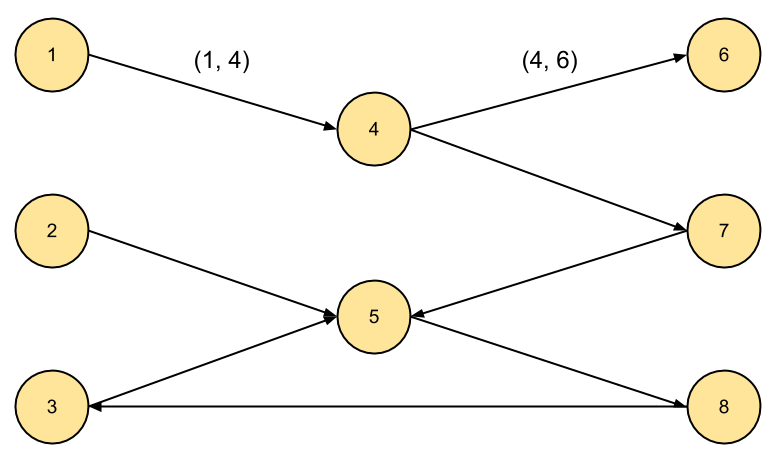
\includegraphics[height=7.5cm]{./chapters/1-intro/figs/node-arcs.png}
  \caption{An example node-arc network configuration. Arrows denote possible
    flow directions. Arc notation examples are provided for arcs (1,4) and
    (4,6).}
  \label{fig:node-arcs}
  \end{center}
\end{figure}

The actual formulation for a network flow problem as a linear program is, of
course, dependent on the problem being modeled. Take for example a maximum flow
problem. The objective of such a problem is to maximize the flow in a system,
i.e.,

\begin{equation}
\max \sum_{(i, j) \in A} x_{i,j}.
\end{equation}

The constraint matrix in such problems is denoted a \textit{node-arc incidence}
matrix. For a directed graph, an arc leaving node $i$ and entering arc $j$
indicates a value of 1 for element $a_{i,j}$ and a value of -1 for element
$a_{j,i}$. If an arc between two nodes does not exist, then a value of 0 is
assigned for the two corresponding coefficients. In general network flow
problems, there is also a notion of \textit{divergence}. Divergence is the total
amount of flow exiting or entering a node, and is modeled by the $b$ vector in
the matrix formulation of network flow problems. As is perhaps obvious, if $b_i
> 0$ for some node, $i$, then more flow exits the node than enters it and it is
termed a \textit{source node}. If $b_i < 0$, then more flow enters the node than
flows in, thus it is termed a \textit{sink node}. Finally, if $b_i = 0$, then
all material that flows into the node flows out as well, and it is termed a
\textit{transshipment node}. Finally, arcs can have their flow bounded, where a
lower bound for arc $(i, j)$ is given as $l_{i,j}$ and an upper bound is denoted
$u_{i,j}$.

One can now construct the LP formulation for a max-flow network flow problem.

%%% 
\begin{subequations}\label{eqs:max-flow}
  \begin{align}
    %%
    \max_{x} \:\: & 
    \sum_{(i, j) \in A} x_{i,j}
    & \label{eqs:max-flow_obj} \\
    %%
    \text{s.t.} \:\: &
    \sum_{j:(i,j) \in A} x_{i,j} - \sum_{i:(i,j) \in A} x_{i,j} = b_i
    & \forall i \in N \label{eqs:max-flow_sup} \\
    %%
    &
    l_{i,j} \leq x_{i,j} \leq u_{i,j}
    & \forall (i, j) \in A \label{eqs:max-flow_x}
    %%
  \end{align}
\end{subequations}
%%% 

\subsubsection{Transportation Problems}
Transportation problems are a subset of the network flow problems and can
therefore be modeled using linear programming. Transportation problems model the
flow of a commodity between source nodes and sink nodes, i.e., there are no
transshipment nodes in the general transportation problem. Critically, this
simplification allows for the nodes in the transportation problem to be
categorized into two explicit groups, sources and sinks. In other words, source
nodes and sink nodes comprise two distinct subsets, $N_1, N_2$, the union of
which comprises all nodes in the transportation graph, $N$. These properties can
be described in set notation.

\begin{equation}
  N_1 \subset N
\end{equation}

\begin{equation}
 N_2 \subset N
\end{equation}

\begin{equation}
  N_1 \cup N_2 = N
\end{equation}

From the node-arc graph point of view, this strict subset division allows for
the transportation problem to be modeled as a \textit{bipartite} graph.

\begin{figure}[H]
  \begin{center}
    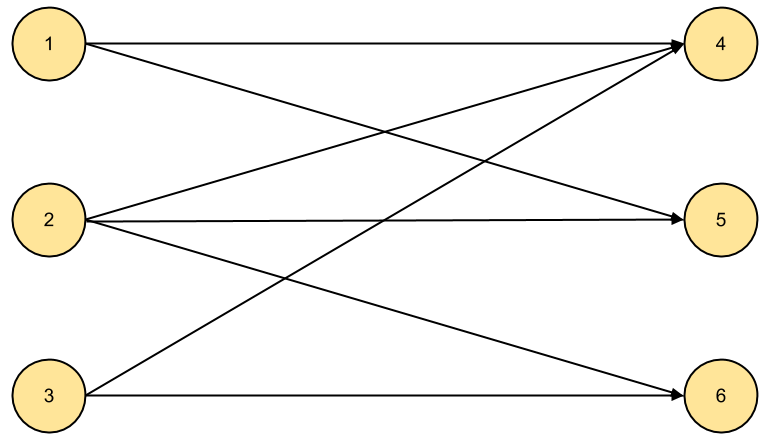
\includegraphics[height=7.5cm]{./chapters/1-intro/figs/node-arcs-bipartite.png}
  \caption{An example node-arc transportation network configuration. Arrows
    denote possible flow directions. Note that all nodes either belong to the 
    set of sources (left) or set of sinks (right).}
  \label{fig:node-arcs-bipartite}
  \end{center}
\end{figure}

The transportation problem is a platform on which one can model more general
problems. The minimum-cost transportation problem is a useful example. In such a
formulation, each arc has an associated \textit{unit cost} associated with the
cost of transporting a unit of a commodity along it, $c_{i,j}$. Additionally,
instead of the notion of divergence, supplier and consumer nodes have an
associated supply, $s_i$, or demand, $d_i$, which provide a notion
of \textit{node capacity} rather than arc capacity.

Accordingly, the minimum-cost transportation problem can be formulated as a
linear program in the following manner.

%%% 
\begin{subequations}\label{eqs:xport}
  \begin{align}
    %%
    \min_{x_{i,j}} \:\: & 
    \sum_{(i, j) \in A \subset N_1 \times N_2} c_{i,j} x_{i,j}
    & \label{eqs:xport_obj} \\
    %%
    \text{s.t.} \:\: &
    \sum_{j \in N_2} x_{i,j} \leq s_i
    & \forall i \in N_1  \\
    %%
    &
    \sum_{i \in N_1} x_{i,j} \geq d_i
    & \forall j \in N_2  \\
    %%
    &
    x_{i,j} \geq 0
    & \forall i \in N_1, \: \forall j \in N_2 \label{eqs:xport_x}
    %%
  \end{align}
\end{subequations}
%%% 

As is noted in many texts on the Transportation Problem Linear Program
formulation, an intuitive constraint on the problem to guarantee a feasible
solution is that the total demand in the system must be no greater than the
total supply in the system.

\begin{equation}
  \sum_{j \in N_2} d_j \leq \sum_{i \in N_1} s_i
\end{equation}

Feasibility in this sense can be guaranteed, however, by adding an artificial
supply node. Such a node can have infinite supply capacity but at (effectively)
infinite cost. The problem can then be solved, and any flow leaving the
artificial node in the optimal solution can be dealt with accordingly, e.g., it
can be ignored.

\subsubsection{Multi-Commodity Transportation Problems}\label{sec:MCTP}
The previously-described transportation problem can more precisely be named the
single-commodity transportation problem. It deals with the flow from sources to
sinks of a single commodity. A more complex model includes more than one
commodity.

Variables and constants in the multi-commodity formulation are generally analogs
of their counterparts in the single-commodity problem. There is a unit cost for
commodity $h$ to traverse arc $(i,j)$ denoted as $c_{i,j}^{h}$. A supplier of
commodity $h$ has a certain supply capacity $s_i^h$ which cannot be surpassed
and demanders of commodity $h$ have a certain demand level which must be met,
$d_i^h$.

In the simplest extension from the single-commodity to multi-commodity
transportation problem, arc constraints for all commodities are combined, i.e.,
for a given arc $(i, j)$, there is a single capacity $u_{i,j}$. A classic
interpretation of this enhanced complexity deals with data networks. Multiple
classifications of data exist, but they all must traverse the same network
infrastructure. Accordingly, the infrastructure can only accommodate a certain
level of total flow among all communication types.

This coupling of commodities via arc capacities changes the structure of the
node-arc incidence matrix. Arc capacity constraints no longer have a single
entry. Instead, many flows contribute to the capacity constraint, requiring
different methods to solve the problem. Of course, the Simplex Method can still
solve the linear program, however other potential reductions in time and
complexity that are available to the single-commodity flow problem are not
available to the multi-commodity flow problem due to this coupling.

The formulation of the multi-commodity flow problem is shown in Equation
\ref{eqs:MCTP}. Note the commodity coupling in Equation \ref{eqs:MCTP_cap}.

%%% 
\begin{subequations}\label{eqs:MCTP}
  \begin{align}
    %%
    \min_{x_{i,j}^{h}} \:\: & 
    \sum_{i \in I}\sum_{j \in J}\sum_{h \in H} c_{i,j}^{h} x_{i,j}^{h}
    & \label{eqs:MCTP_obj} \\
    %%
    \text{s.t.} \:\: &
    \sum_{j \in J} x_{i,j}^{h} \leq s_{i}^{h}
    &
    \forall \: i \in I, \forall \: h \in H \label{eqs:MCTP_sup} \\
    %%
    &
    \sum_{i \in I} x_{i,j}^{h} \geq d_{j}^{h}
    & 
    \forall \: j \in J, \forall \: h \in H \label{eqs:MCTP_dem} \\
    %%
    &
    \sum_{h \in H} x_{i,j}^{h} \leq u_{i,j}
    & 
    \forall \: j \in J \label{eqs:MCTP_cap} \\
    %%
    &
    x_{i,j}^{k} \geq 0
    &
    \forall \: i \in I, \forall \: j \in J, \forall \: h \in H \label{eqs:MCTP_x}
    %%
  \end{align}
\end{subequations}
%%% 

A number of important reductions are possible for the multi-commodity
transportation problem, e.g., the case in which is no arc that shares multiple
commodities. In this instance the multicommodity connection constraints
disappear, and the single multi-commodity problem can be broken into $m$
different single-commodity transportation problems, where $m$ is the cardinality
of the set of commodities, $H$. 

These simplifications are important to the computation time required to solve
the resulting problem instance. The general solution technique for LPs is the
Simplex Method, as previously described. Klee and Minty show that in the worst
case, the Simplex Method will execute in exponential time \cite{klee_good_1970},
but in practice it is generally considered very computationally efficient. If
the problem can be simplified to a TP, then the Transportation Simplex Method
can be used \cite{ahuja_network_1993}.

In general, optimization problems are solved by solving a number of decision
problems. Decision problems are generally computationally
\textit{hard}. Decision problems ask yes or no questions, e.g., ``is there a
flow path that with a flow larger than $x$?''. An optimization problem asks
instead ``what is the flow path with the largest flow?''. Any problem can be
associated with one of four categories of computational complexity:

\begin{itemize}
        \item Polynomial-time ($\mathcal{P}$)
        \item Nondeterministic Polynomial-time ($\mathcal{NP}$)
        \item Nondeterministic Polynomial-time Complete  ($\mathcal{NP}$-C)
        \item Nondeterministic Polynomial-time Hard  ($\mathcal{NP}$-hard)
\end{itemize}

The topic of computational complexity is relatively involved, thus I will only
provide a short overview to provide context. A problem is considered to reside
in $\mathcal{P}$ if there is a polynomial-time algorithm that can solve it. A
classic example is that of naive matrix inversion, known to be of order $n^3$
(i.e., $\mathcal{O}(n^3)$) for a given $n \times n$ matrix.

A decision problem is considered to be in ($\mathcal{NP}$) if for any proposed
solution, there is a \textit{short certificate}.

\begin{define}
A \textbf{certificate} is a method to verify that a solutions provides a
positive or negative response to the question at hand. A certificate is
considered \textbf{short} if it is polynomial in size and can be verified in
polynomial time.
\end{define}

A decision problem, $Q$, is considered to be in $\mathcal{NP}$-C, if
$Q \in \mathcal{NP}$ and \textit{any} problem, $P \in \mathcal{NP}$ is
polynomial-time reducible to $Q$, i.e., instances of $P$ can be reformulated as
instances of $Q$ in polynomial time. The most popular candidate of this
polynomial reduction is the Satisfiability Problem, known to be in
$\mathcal{NP}$-C.

Finally, a problem $Q$, is in $\mathcal{NP}$-hard, if any problem
$P \in \mathcal{NP}$ is polynomial-time reducible to $Q$, but
$Q \not\in \mathcal{NP}$. If a decision problem is in $\mathcal{NP}$-C, then the
corresponding optimization problem is $\mathcal{NP}$-hard.

The various levels of complexity are related. It is not known whether
$\mathcal{P} = \mathcal{NP}$, but it is strongly suspected that
$\mathcal{P} \subset \mathcal{NP}$. It is also assumed that
$\mathcal{NP}\text{-C} \subset \mathcal{NP}$, and
$\mathcal{NP}\text{-hard} \notin \mathcal{NP}$ by definition. The relationship
between these set of problem complexities is shown graphically in
Figure \ref{fig:complexity}.

\begin{figure}[H]
  \begin{center}
    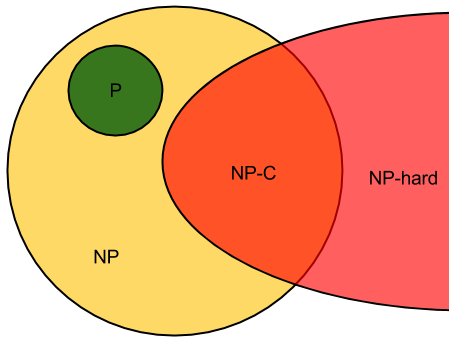
\includegraphics[height=7.5cm]{./chapters/1-intro/figs/complexity.png}
  \caption{The relationship between the various types of problem complexities.}
  \label{fig:complexity}
  \end{center}
\end{figure}
